\chapter{Tillämpningar av integraler}
Vi har följande geometriska tolkning av integraler:\\
$\int_a^bf(x)\, dx=$"arean med tecken under grafen till $f(x)$ begränsad av $x$-axeln"\\
%infoga bild 1
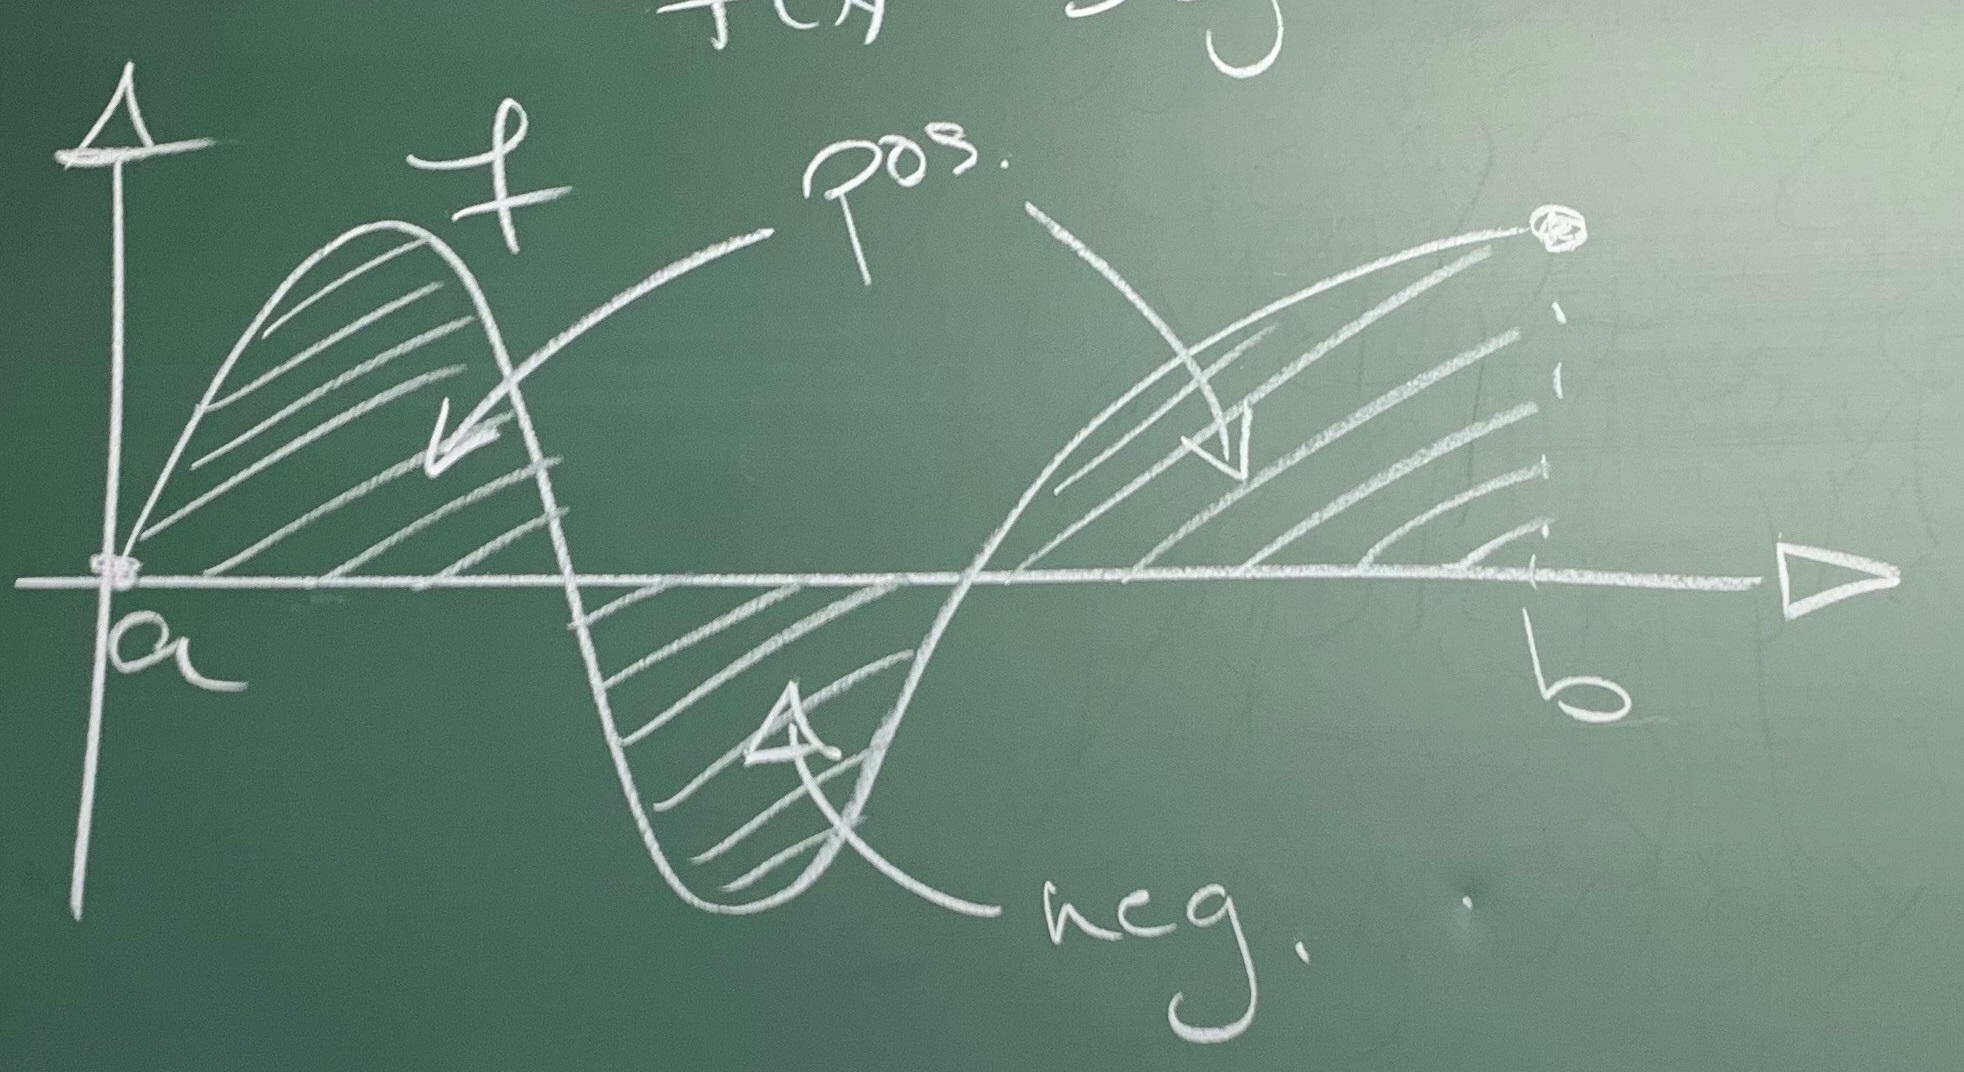
\includegraphics[scale=0.1]{lessons/lesson19/imgs/img01.jpg}
Om man vill ha totalarean (dvs arean utan tecken) är det bara att integrera $|f(x)|$ istället.
\begin{equation*}
    \int_a^b|f(x)|\, dx=\text{"totala arean under grafen"}
\end{equation*}
På liknande sätt kan man beräkna arean mellan två grafer.
%infoga bild 2
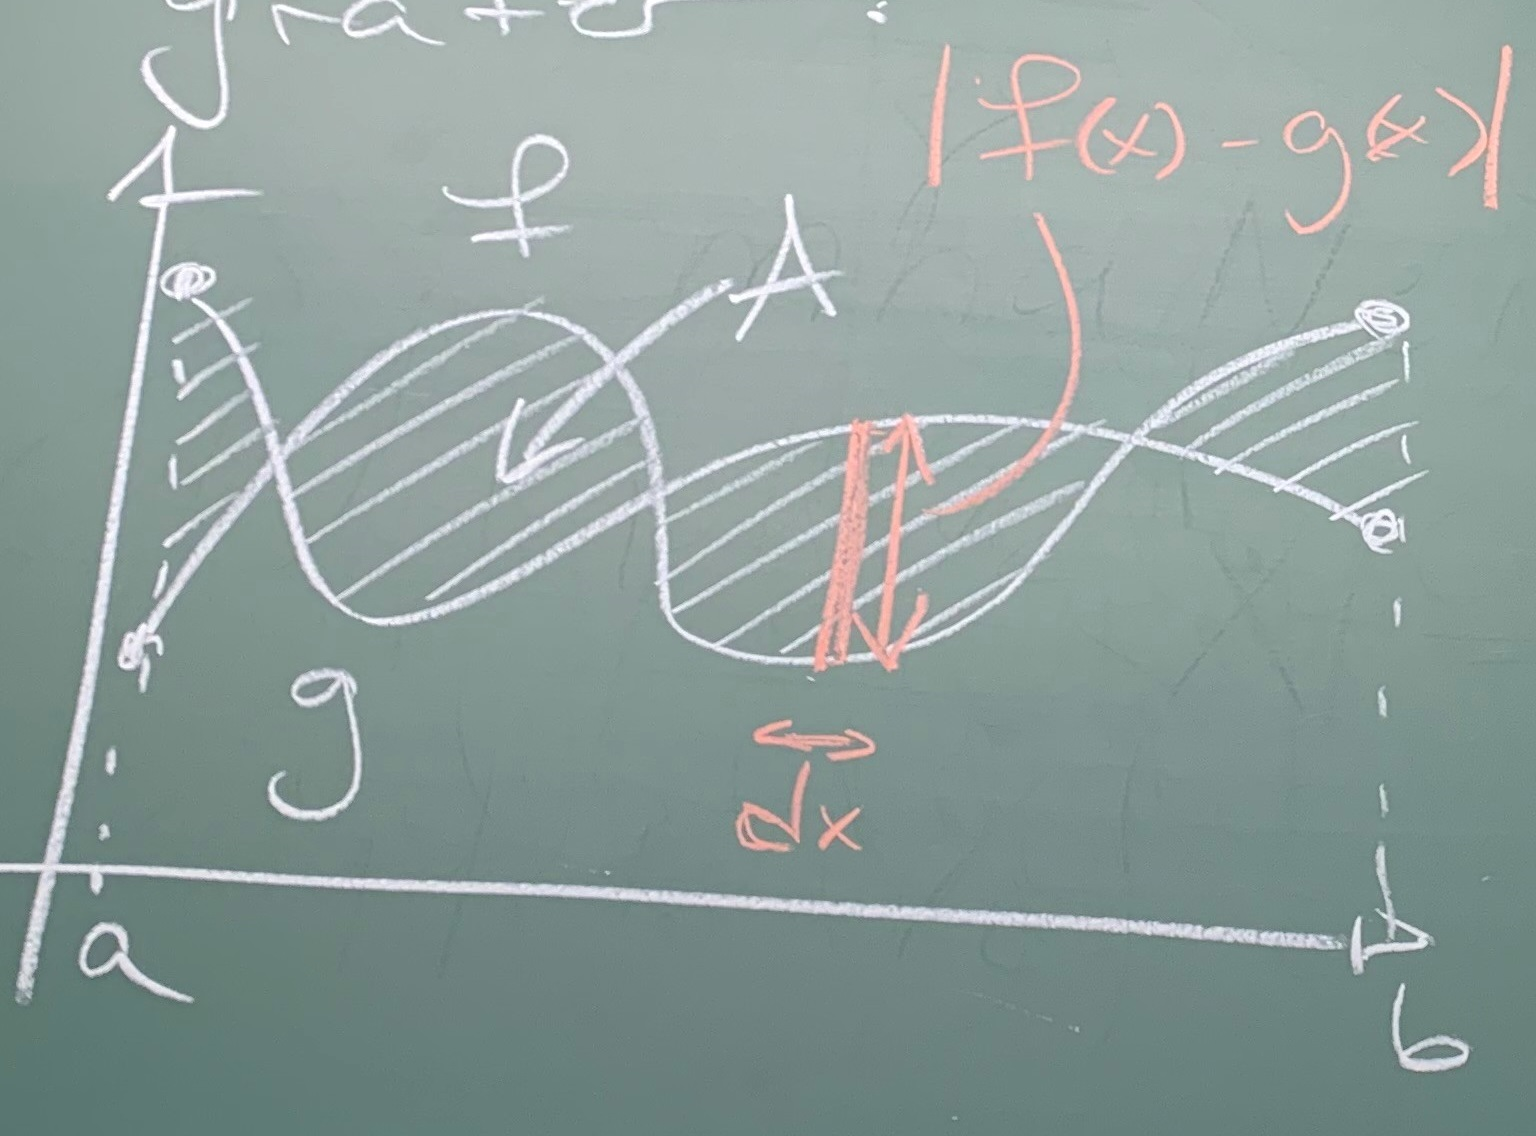
\includegraphics[scale=0.1]{lessons/lesson19/imgs/img02.jpg}
\begin{equation*}
    A=\int_a^b|f(x)-g(x)|\, dx
\end{equation*}
Metoden med att integrera infinitesimala element, som till exempel $|f(x)-g(x)|\,dx$, är mycket användbar.

\section{Volymberäkning}
Att beräkna volymer med integraler kräver i allmänhet teori från från flervariabelanalys eftersom det grundläggande infinitesimala elementet är en liten kub med volym $dV=dx\,dy\,dz$.
%infoga bild 3
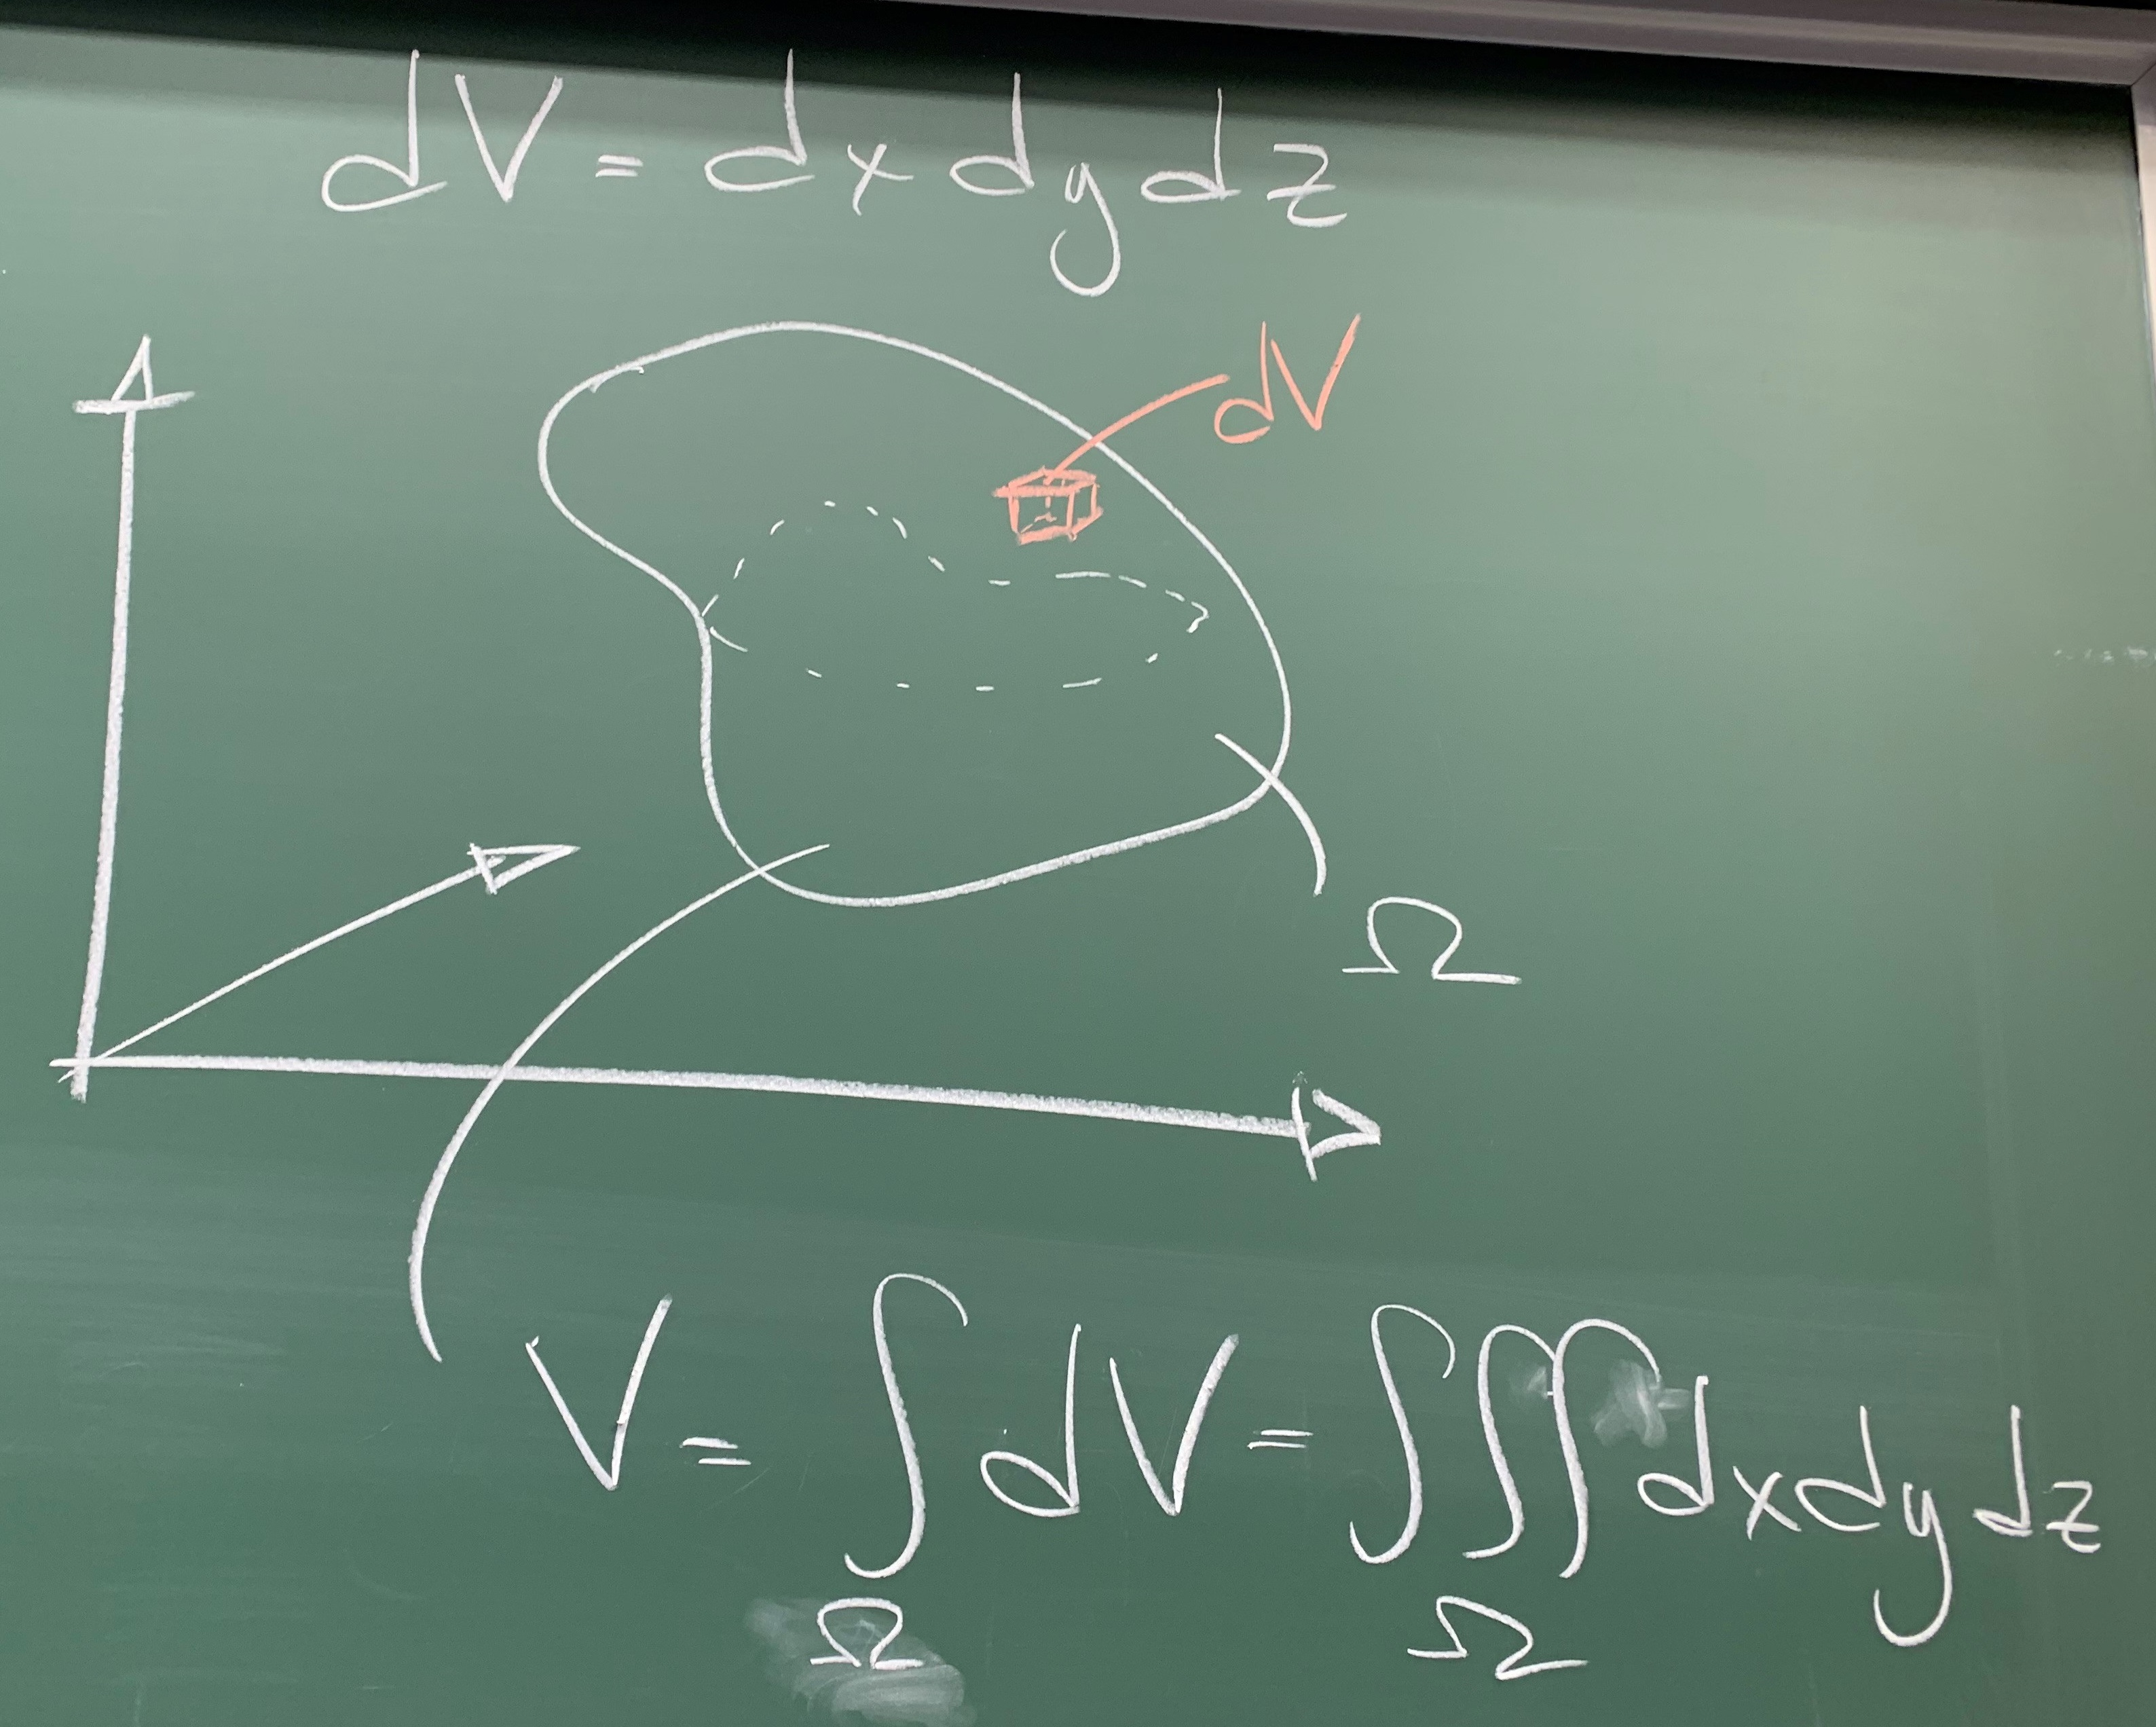
\includegraphics[scale=0.1]{lessons/lesson19/imgs/img03.jpg}
Ibland klarar man sig dock med vanliga enkelintegraler om man kan skriva $dV=A(x)dx$, där $A(x)$ beskriver arean av en "skiva" och $dx$ är skivans tjocklek.
Går om volymen man vill beräkna uppvisar någon form av symmetri.
%infoga bild 4
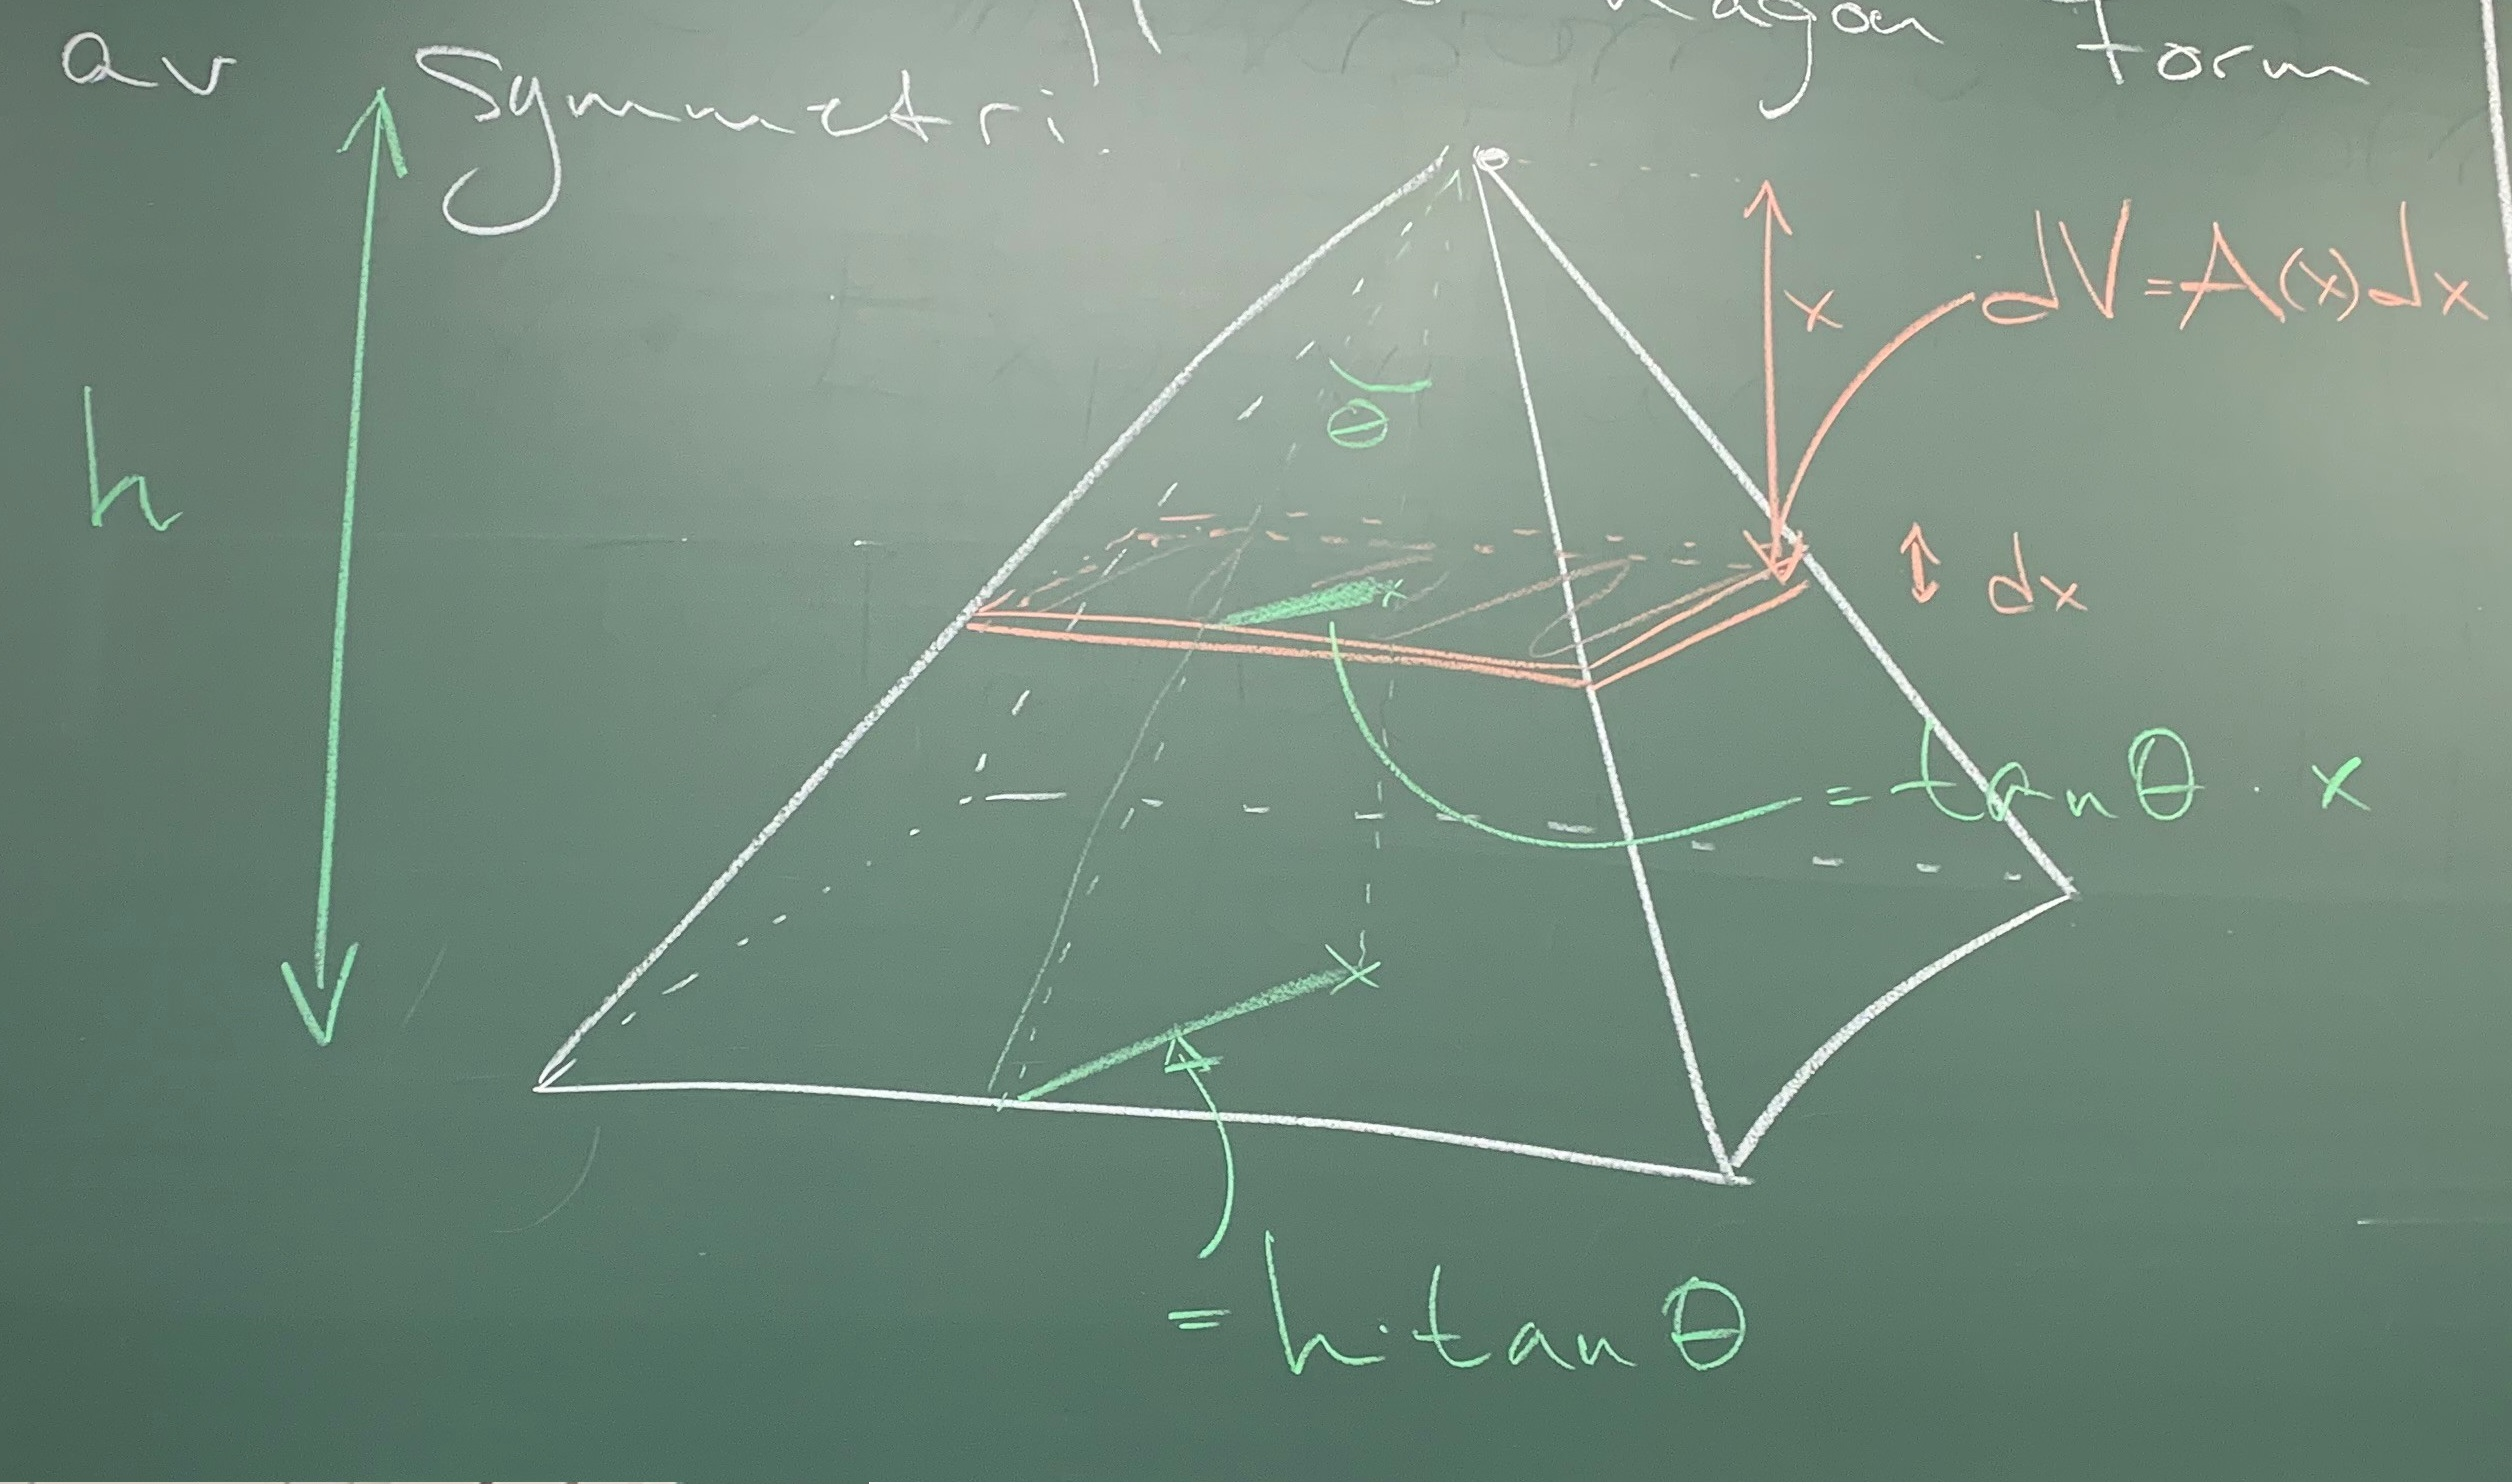
\includegraphics[scale=0.1]{lessons/lesson19/imgs/img04.jpg}
\begin{equation*}
    A(x)=(2\cdot x\cdot\tan(\theta))^2=4x^2\tan^2(\theta)\Rightarrow
    V=\int\, dV=
    \int A(x)\, dx=
\end{equation*}
\begin{equation*}
    \int_0^h 4x^2\tan^2(\theta)\, dx=
        [\frac{4}{3}x^3\tan^2(\theta)]_0^h=
    \frac{4}{3}h^3\cdot\tan^2(\theta)=
    \frac{h}{3}4h^2\tan^2(\theta)=
\end{equation*}
\begin{equation*}
    \{4h^2\tan^2(\theta)="basytan"=b\}=
    \frac{h\cdot b}{3}
\end{equation*}
Ibland uppvisar volymer rotationssymmetri med antingen $x$- eller $y$-axeln och då utnyttjas detta genom rotationssymmetriska element.
%infoga bild 5
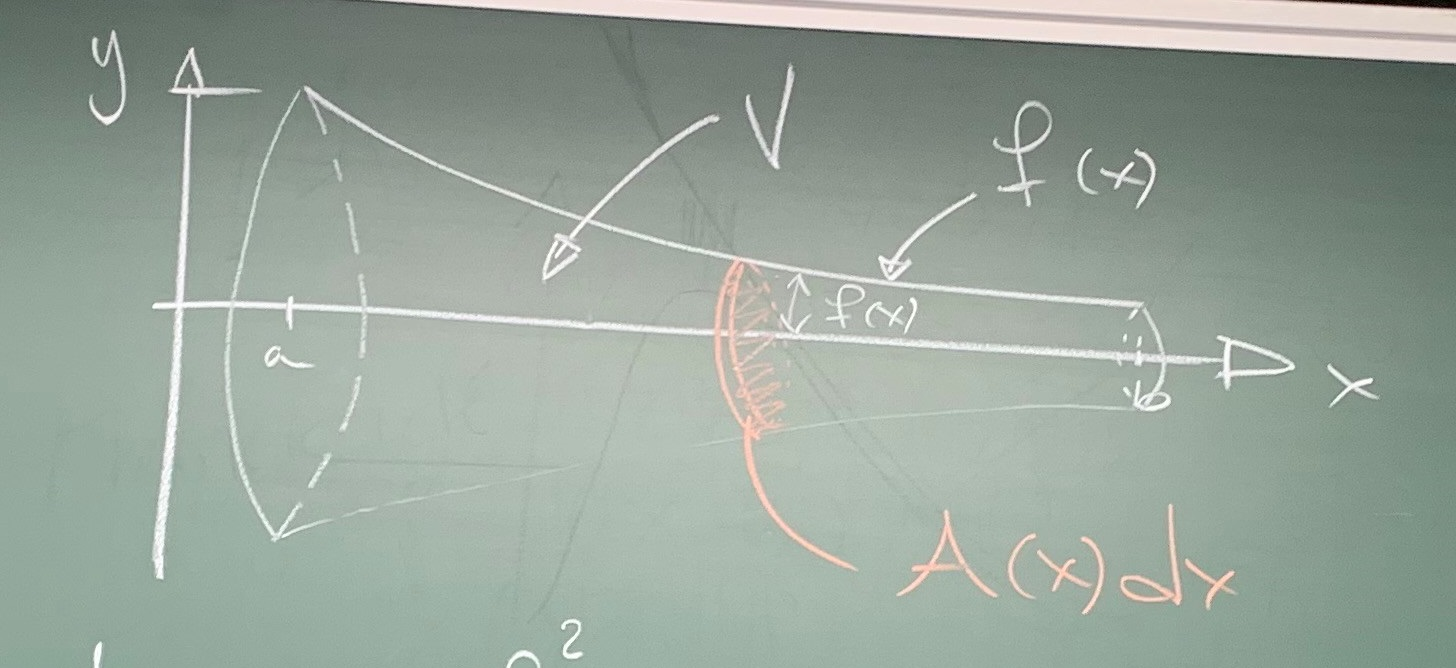
\includegraphics[scale=0.1]{lessons/lesson19/imgs/img05.jpg}
\begin{equation*}
    A(x)=f^2(x)\cdot\pi\Rightarrow
    V=\int dV=\int_a^bf^2(x)\overline{u}\, dx
\end{equation*}
Liknande konstruktion runt $y$-axeln.

\paragraph*{Ex (7.1.16)} Bestäm volymen av den kropp som fås genom att rotera en cirkelskiva runt en godtycklig tangentlinje.
\subparagraph{Lösning}
%infoga bild 6
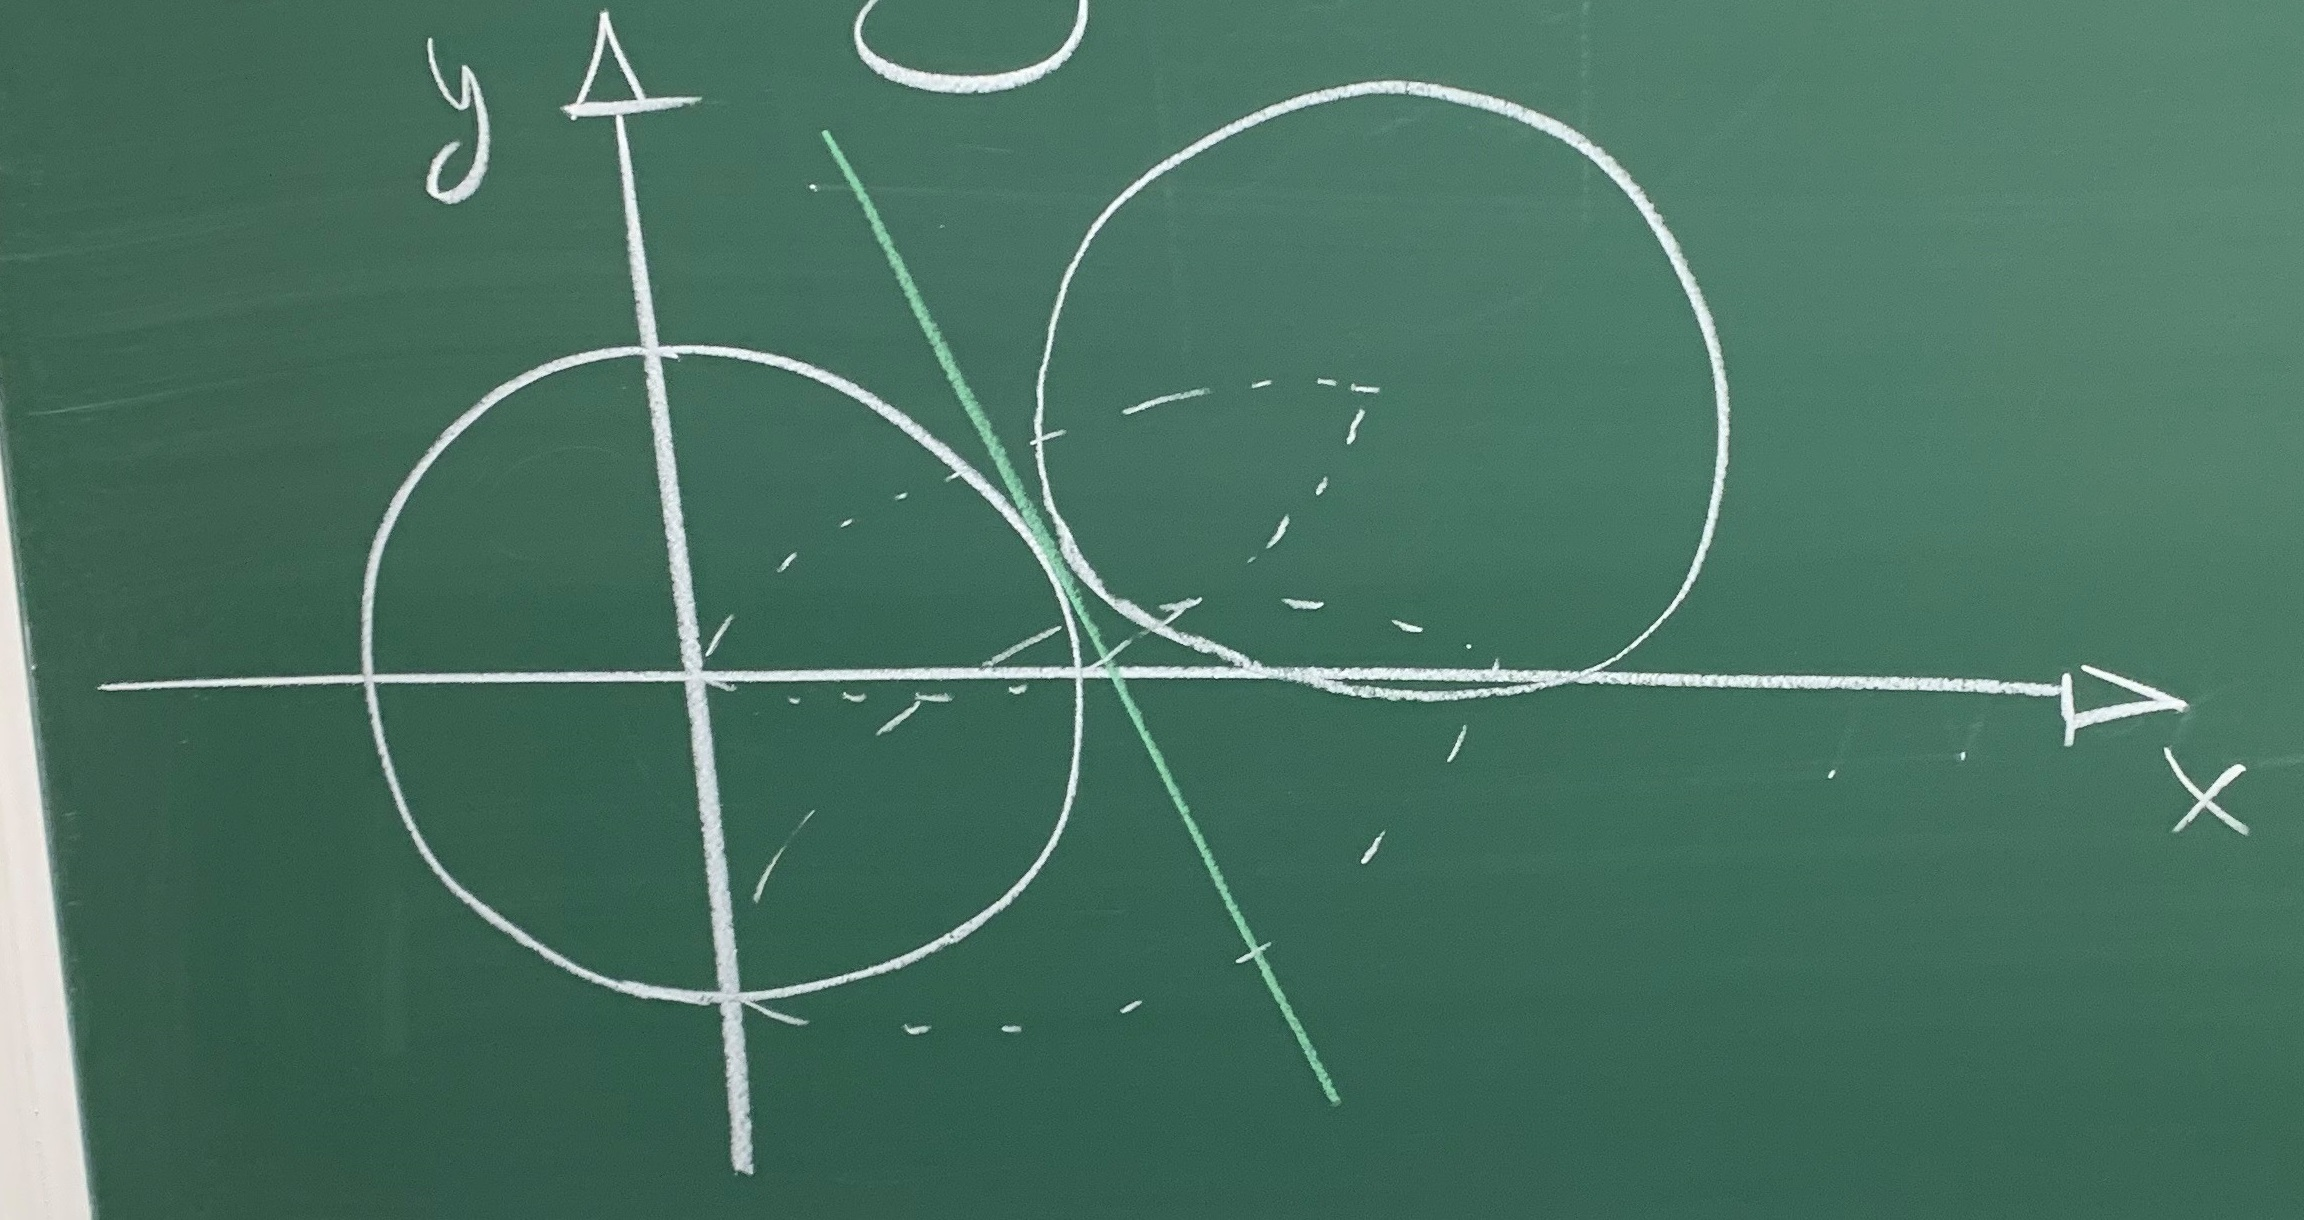
\includegraphics[scale=0.1]{lessons/lesson19/imgs/img06.jpg}
Volymen är av symmetriskäl oberoende av tangentlinje, så välj linjen $x=r$, där $r$ är cirkelskivans radie.
%infoga bild 7
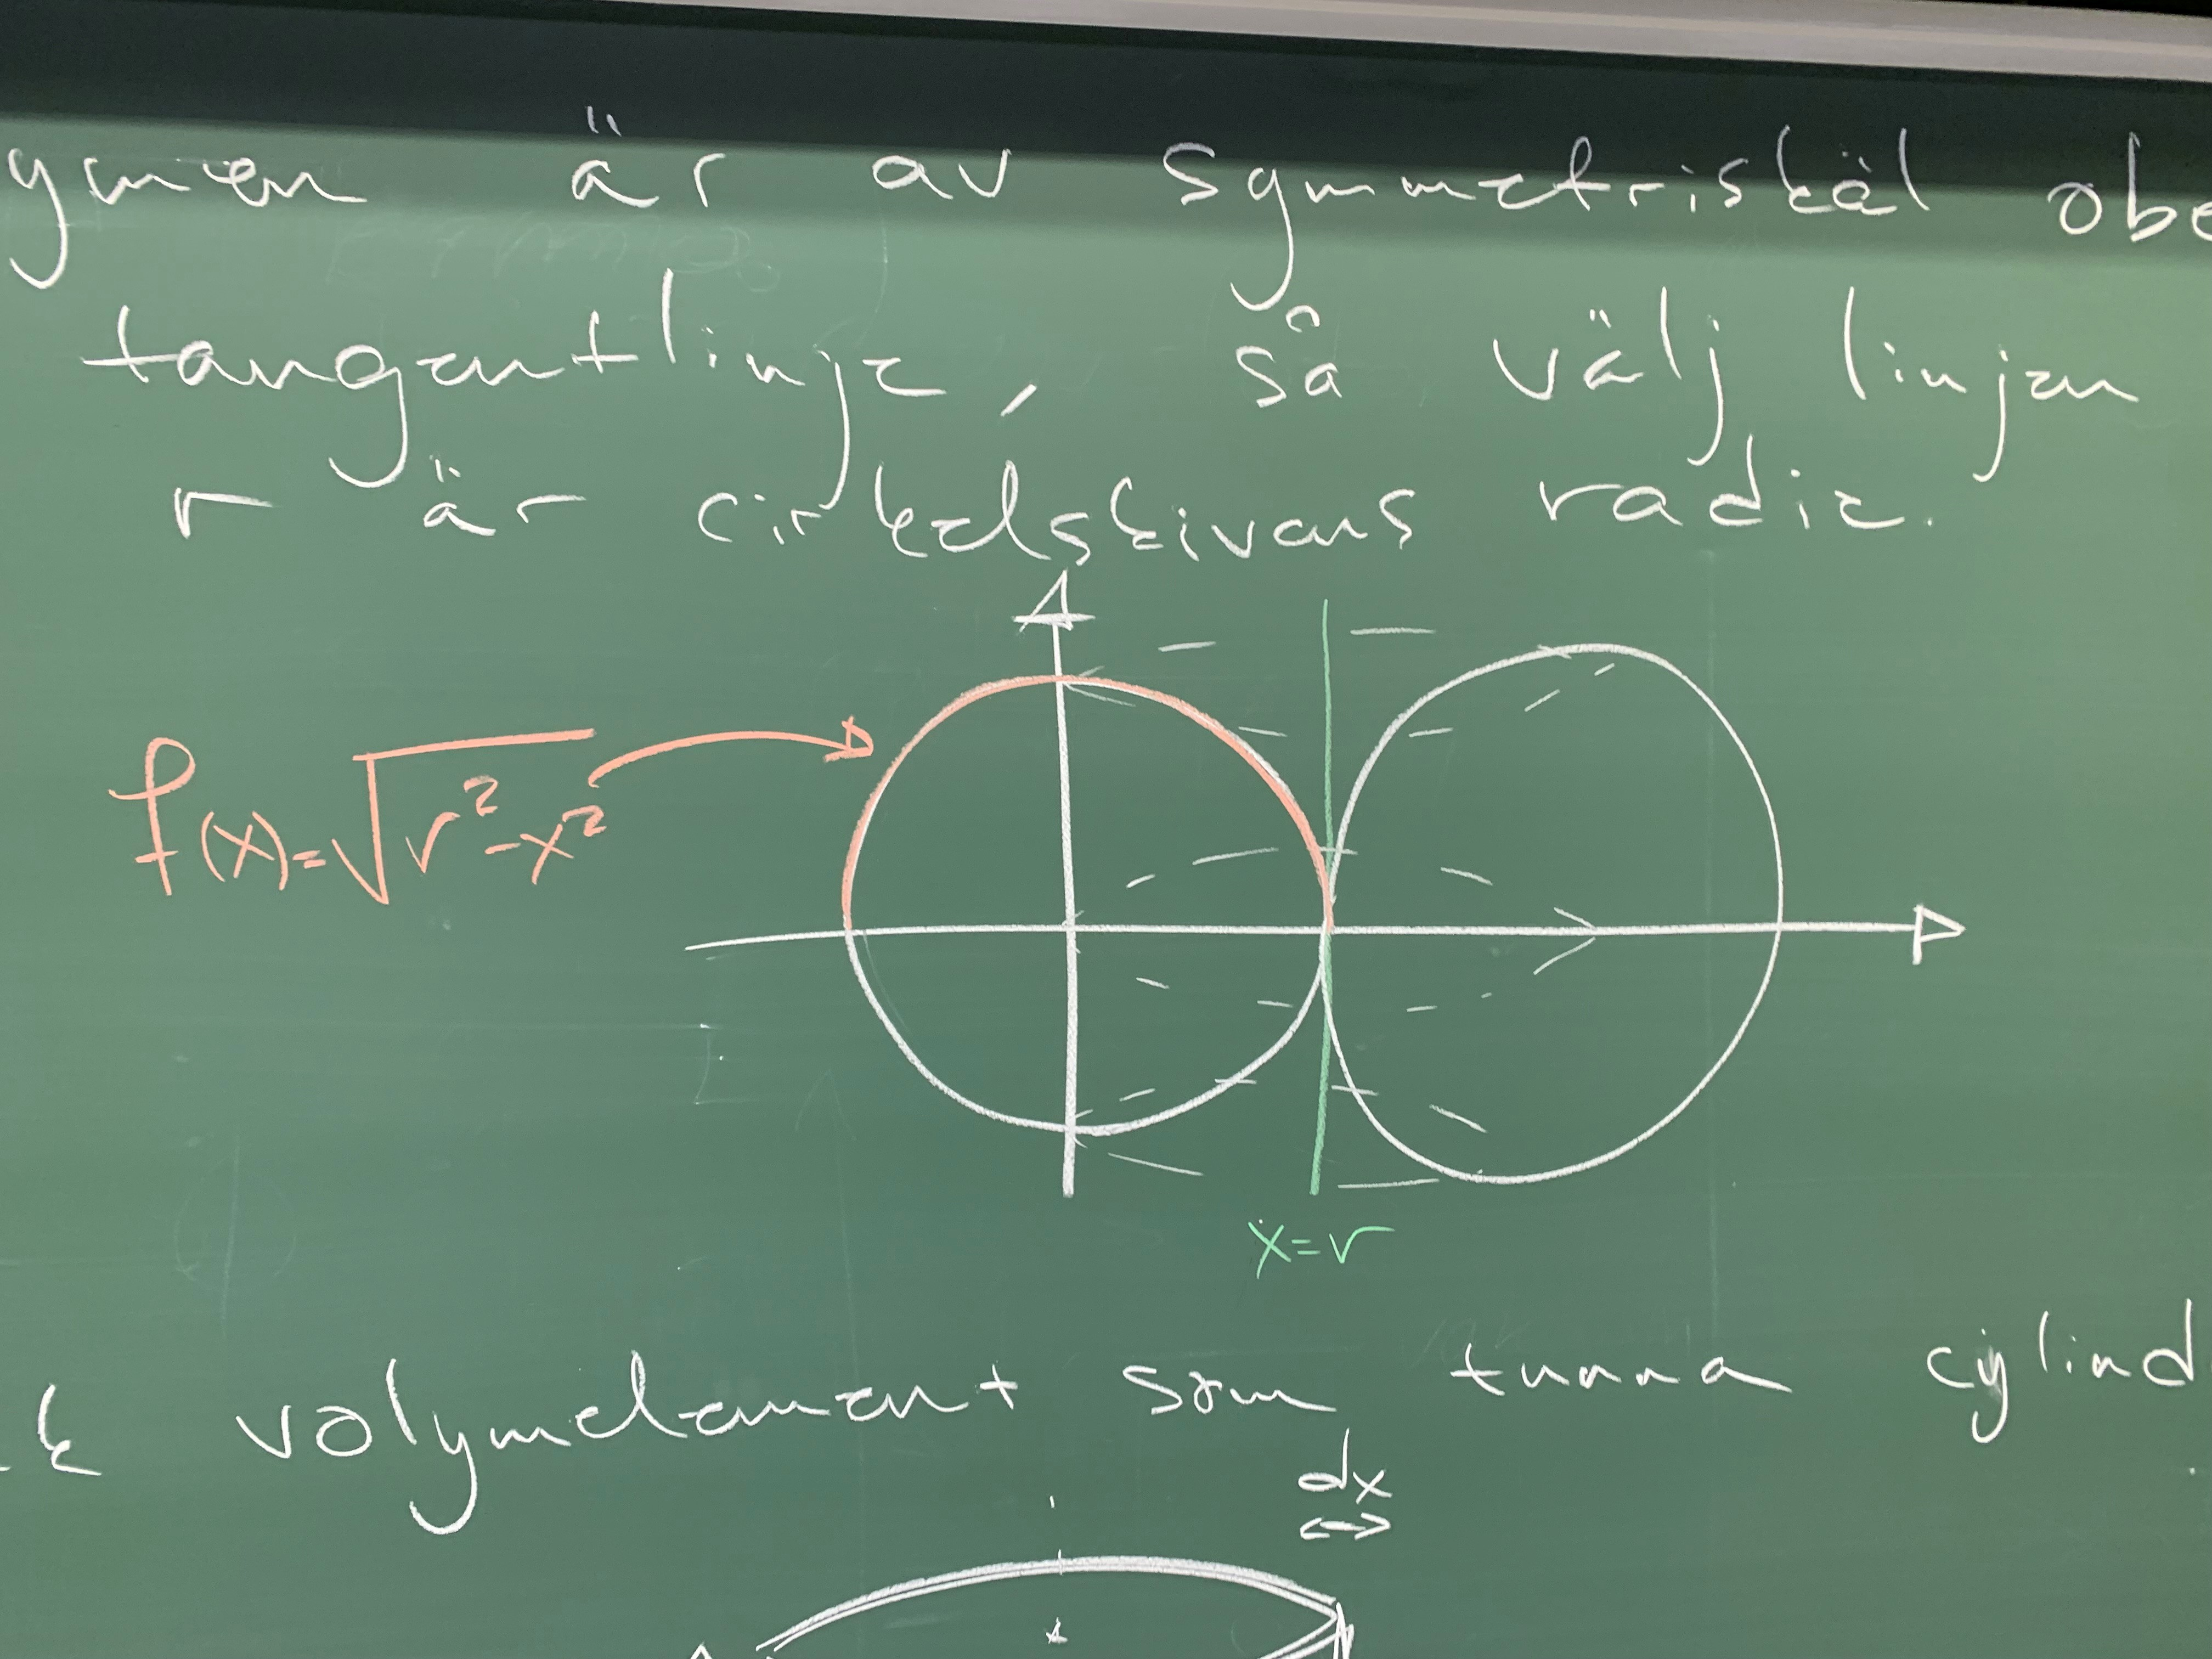
\includegraphics[scale=0.1]{lessons/lesson19/imgs/img07.jpg}
Tänk volym element som tunna cylindrar:
%infoga bild 8
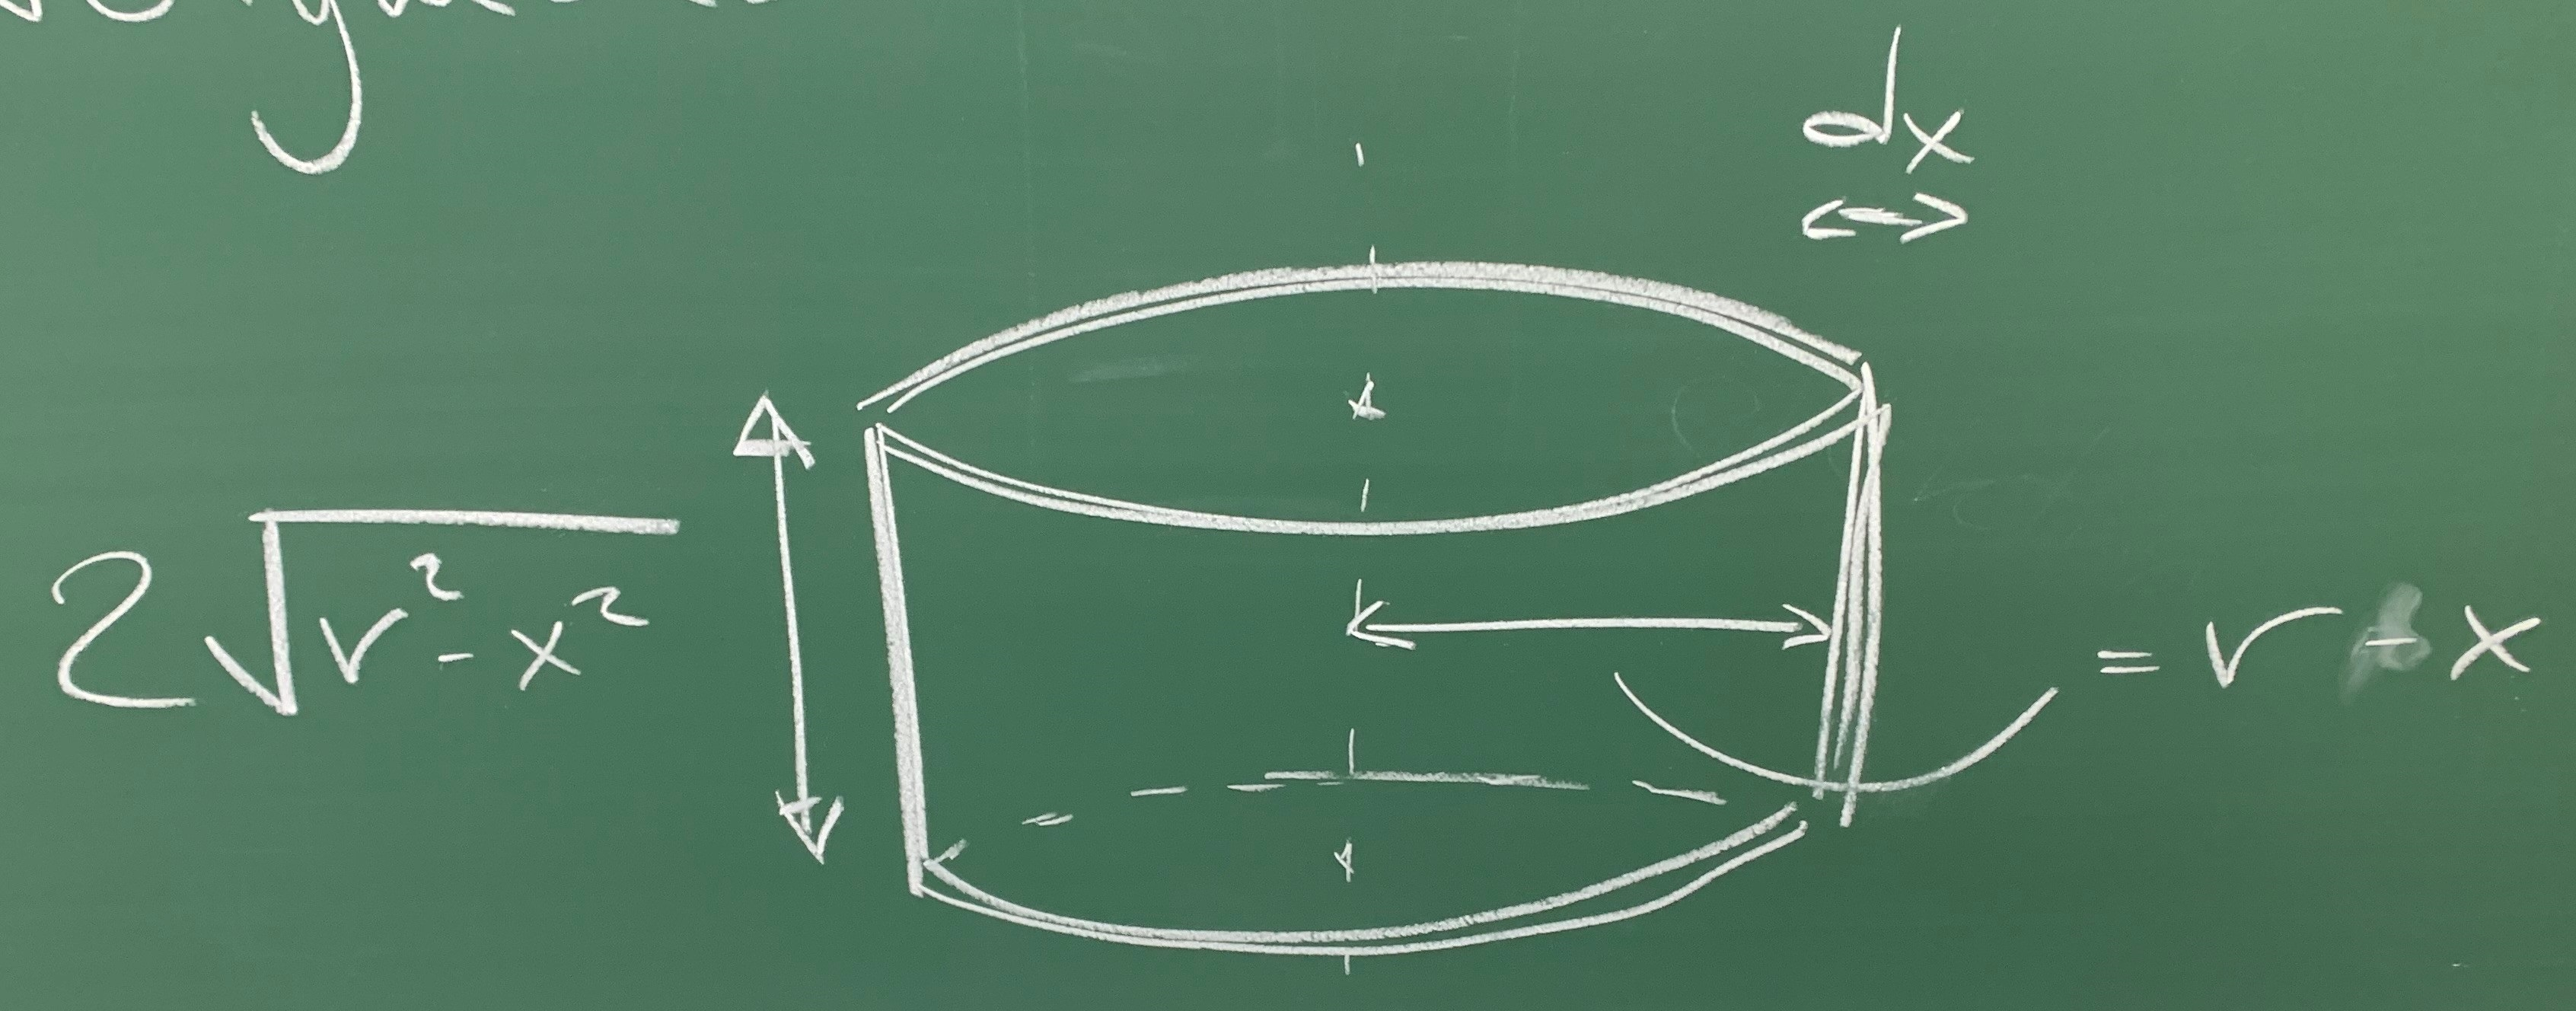
\includegraphics[scale=0.1]{lessons/lesson19/imgs/img08.jpg}
\begin{equation*}
    \rightarrow V=\int dV=\int_{-r}^r A(x)\, dx=
    \int_{-r}^r2\pi(r-x)\cdot 2\sqrt{r^2-x^2}\, dx=
\end{equation*}
\begin{equation*}
    4\pi[r\int_{-r}^r]\sqrt{r^2-x^2}\, dx - \int_{-r}^r x\sqrt{r^2-x^2}\, dx=
    4\pi r\int_{-r}^r\sqrt{r^-x^2}\, dx=
\end{equation*}
\begin{equation*}
    \{\text{arean av halvcirkeln}=\frac{\pi r^2}{2}\}=
    4\pi r\cdot\frac{\pi r^2}{2}=
    2\pi^2r^3 \Box
\end{equation*}

\section{Kurvlängd och mantelarea}
Kan approximera en kurva $C$ genom ett så kallat "polygontåg".\\
%infoga bild 9
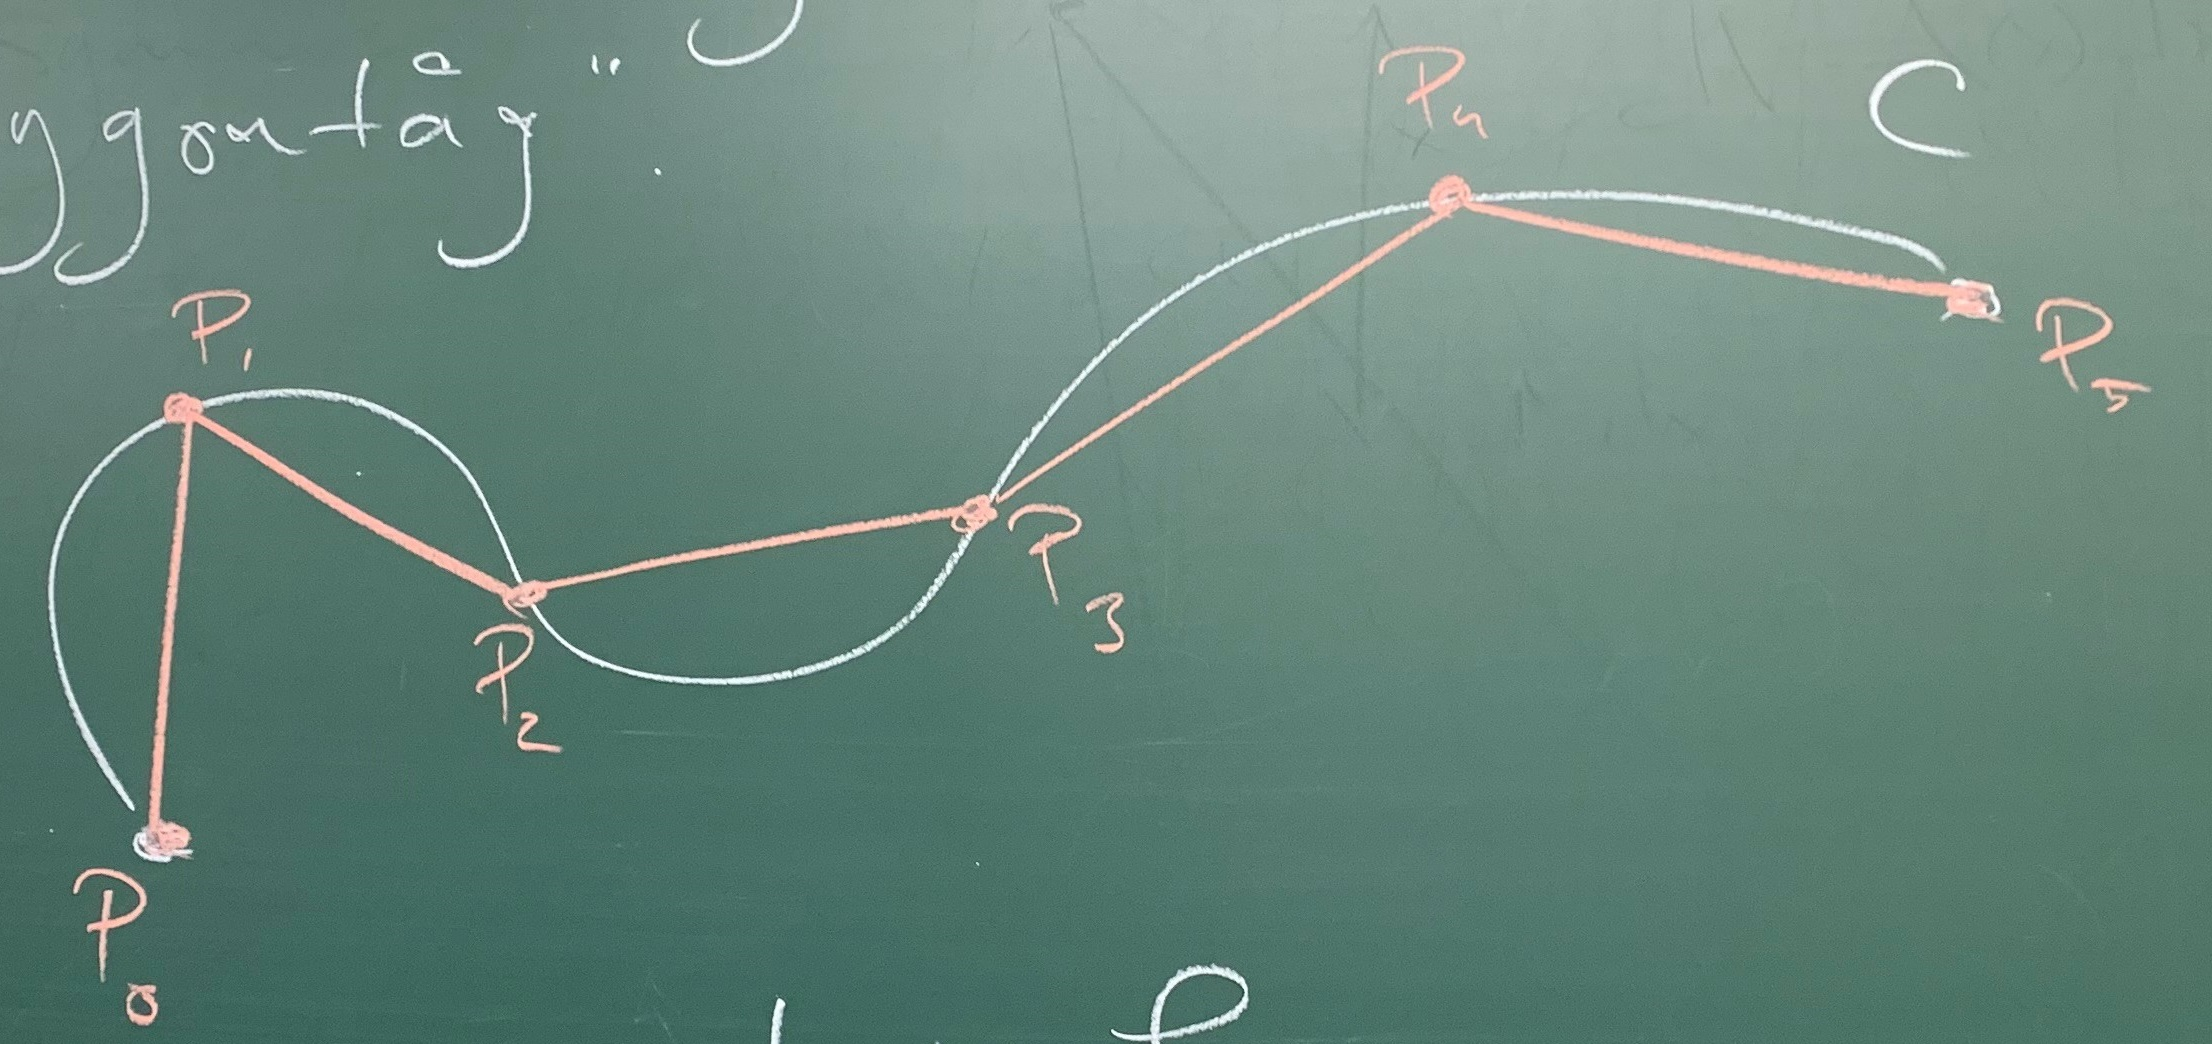
\includegraphics[scale=0.1]{lessons/lesson19/imgs/img09.jpg}
klart att det för varje polygontåg definierat av punkterna $\{P_0,P_1,...,P_n\}$ gäller att dess längd $L_n$ är kortare än den verkliga längden av $C$.
Man \underline{definierar} längden av $C$ som det minsta tal $s\in\mathbb{R}$ så att $L_n\leq s$ för alla polygontåg $\{P_0,P_1,...,P_n\}$.
Längden för ett linjesegment, säg mellan $P_i$ och $P_{i+1}$, blir:
%infoga bild 10
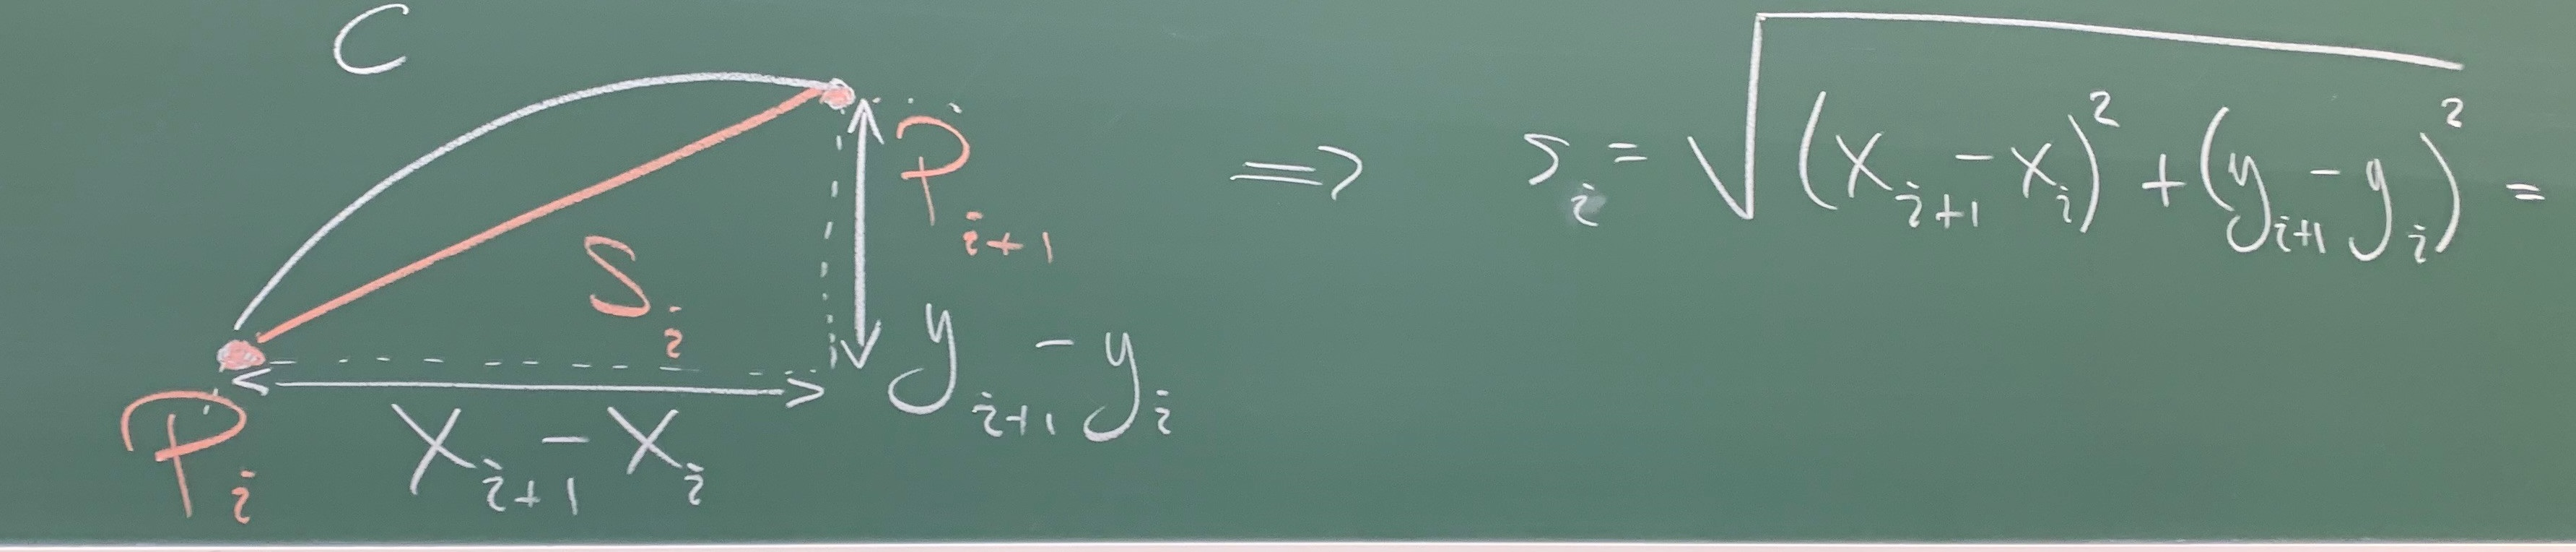
\includegraphics[scale=0.1]{lessons/lesson19/imgs/img10.jpg}
\begin{equation*}
    \Rightarrow s_i=
    \sqrt{(x_{i+1}-x_i)^2+(y_{i+1}-y_i)^2}=
    \sqrt{1+\frac{(y_{i+1}-y_i)^2}{(x_{i+1}-x_i)^2}}\cdot |x_{i+1}-x_i|
\end{equation*}
Om kurvans $y$-värden beskrivs av en funktion $f(x)$, polygontåget blir tätare och tätare och $f^\prime(x)$ existerar
\begin{equation*}
    s_i\to ds=\sqrt{1+(f^\prime(x))^2}\, dx
\end{equation*}
och $s=\int ds=\int_a^b\sqrt{1+(f^\prime(x))^2}\, dx$.

\paragraph*{Ex (7.3.12)} Bestäm längden av kurvan $x=-\frac{1}{2}$ och $x=\frac{1}{2}$ som definieras av grafen till $y=\ln(1-x^2)$.
\subparagraph{Lösning}
Kurvan kan skissas som\\
%infoga bild 11
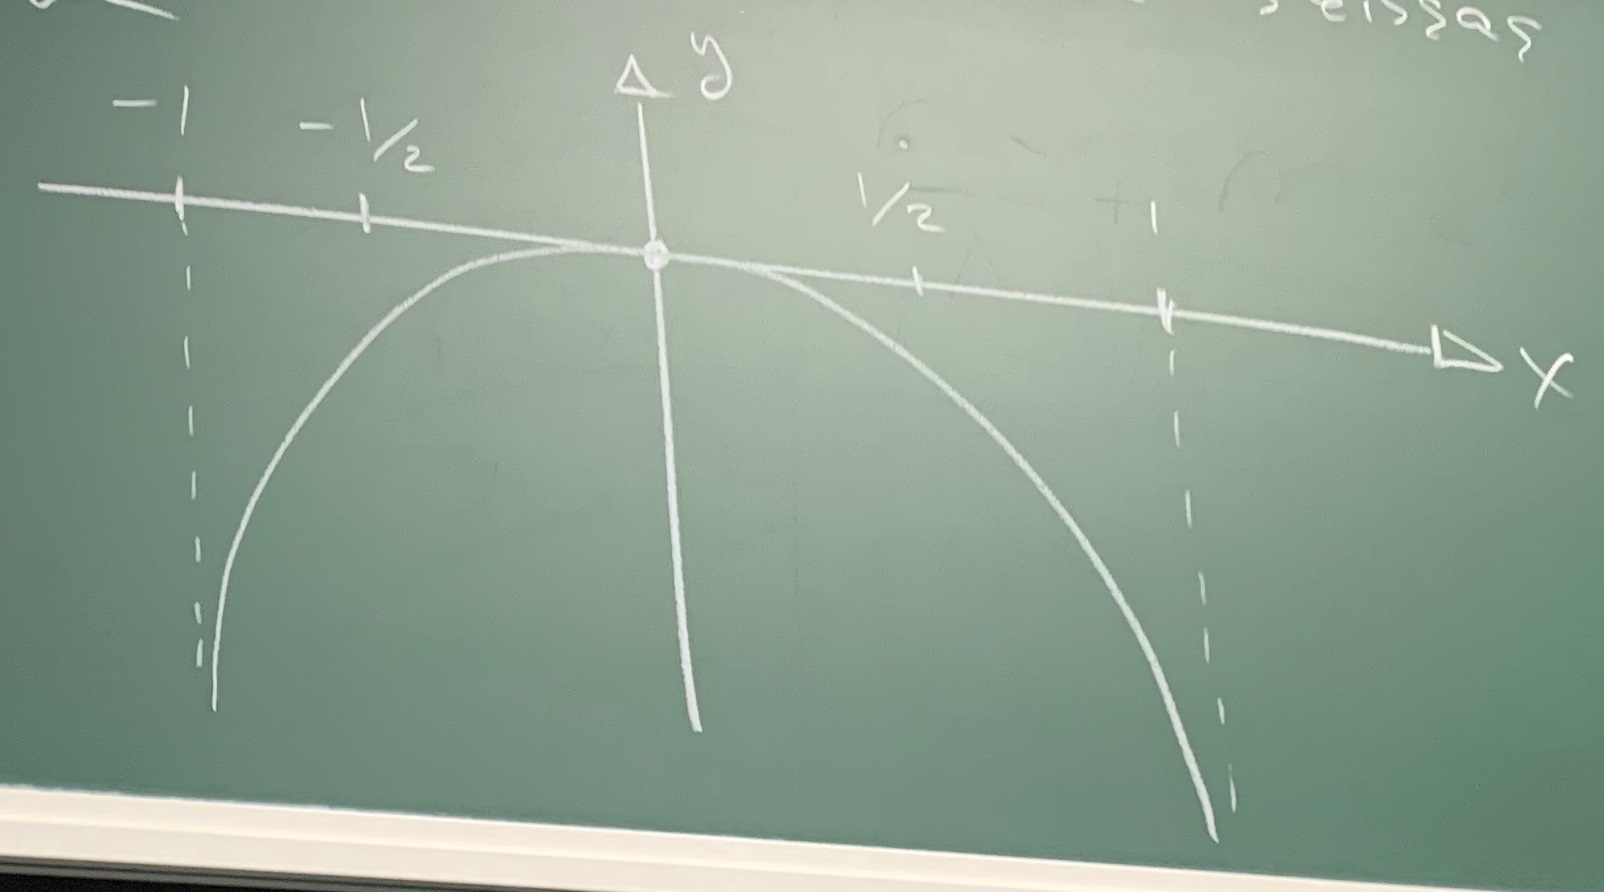
\includegraphics[scale=0.1]{lessons/lesson19/imgs/img11.jpg}
Det gäller att $y^\prime=\frac{1}{1-x^2}\cdot(-2x)=-\frac{2x}{1-x^2}$ för allla $x\in(-\frac{1}{2},\frac{1}{2})$ och alltså kan kurvans längd beräknas som:
\begin{equation*}
    s=\int_{-\frac{1}{2}}^\frac{1}{2}\sqrt{1+(-\frac{2x}{1-x^2})^2}\, dx=
    \int_{-\frac{1}{2}}^\frac{1}{2}\sqrt{1+\frac{4x^2}{(1-x^2)^2}}\, dx=
\end{equation*}
\begin{equation*}
    2\cdot\int_0^\frac{1}{2}\sqrt{1+\frac{4x^2}{(1-x^2)^2}}\, dx=
    2\int_0^\frac{1}{2}\sqrt{\frac{(1-x^2)^2+4x^2}{(1-x^2)^2}}\, dx=
\end{equation*}
\begin{equation*}
    2\int_0^\frac{1}{2}\sqrt{\frac{1-2x^2+x^4+4x^2}{(1-x^2)^2}}\, dx=
    2\int_0^\frac{1}{2}\sqrt{\frac{x^4-2x^2+1}{(1-x^2)^2}}\, dx=
\end{equation*}
\begin{equation*}
    2\int_0^\frac{1}{2}\sqrt{\frac{(x^2+1)^2}{(1-x^2)^2}}\, dx=
    2\int_0^\frac{1}{2}\frac{x^2+1}{1-x^2}=
    2\int_0^\frac{1}{2}\frac{x^2+1+2-2}{1-x^2}=
\end{equation*}
\begin{equation*}
    2\int_0^\frac{1}{2}\frac{2}{1-x^2}-1\, dx=
    \{\frac{2}{1-x^2}=\frac{A}{1+x}+\frac{B}{1-x}\Rightarrow A=B=1\}=
\end{equation*}
\begin{equation*}
    2\int_0^\frac{1}{2}\frac{1}{1+x}+\frac{1}{1-x}-1\, dx=
    2[\ln(|1+x|)-\ln(|1-x|)-x]_0^\frac{1}{2}=
\end{equation*}
\begin{equation*}
    2\cdot(\ln(\frac{3}{2})-\ln(\frac{1}{2})-\frac{1}{2})=
    2\ln(3)-1 \Box
\end{equation*}
Kan använda liknande teknik som för kurvlängder för att beräkna mantelytan av rotationssymmetriska kroppar till exempel om rotationssymmetrin längs $x$-axeln:\\
%infoga bild 12
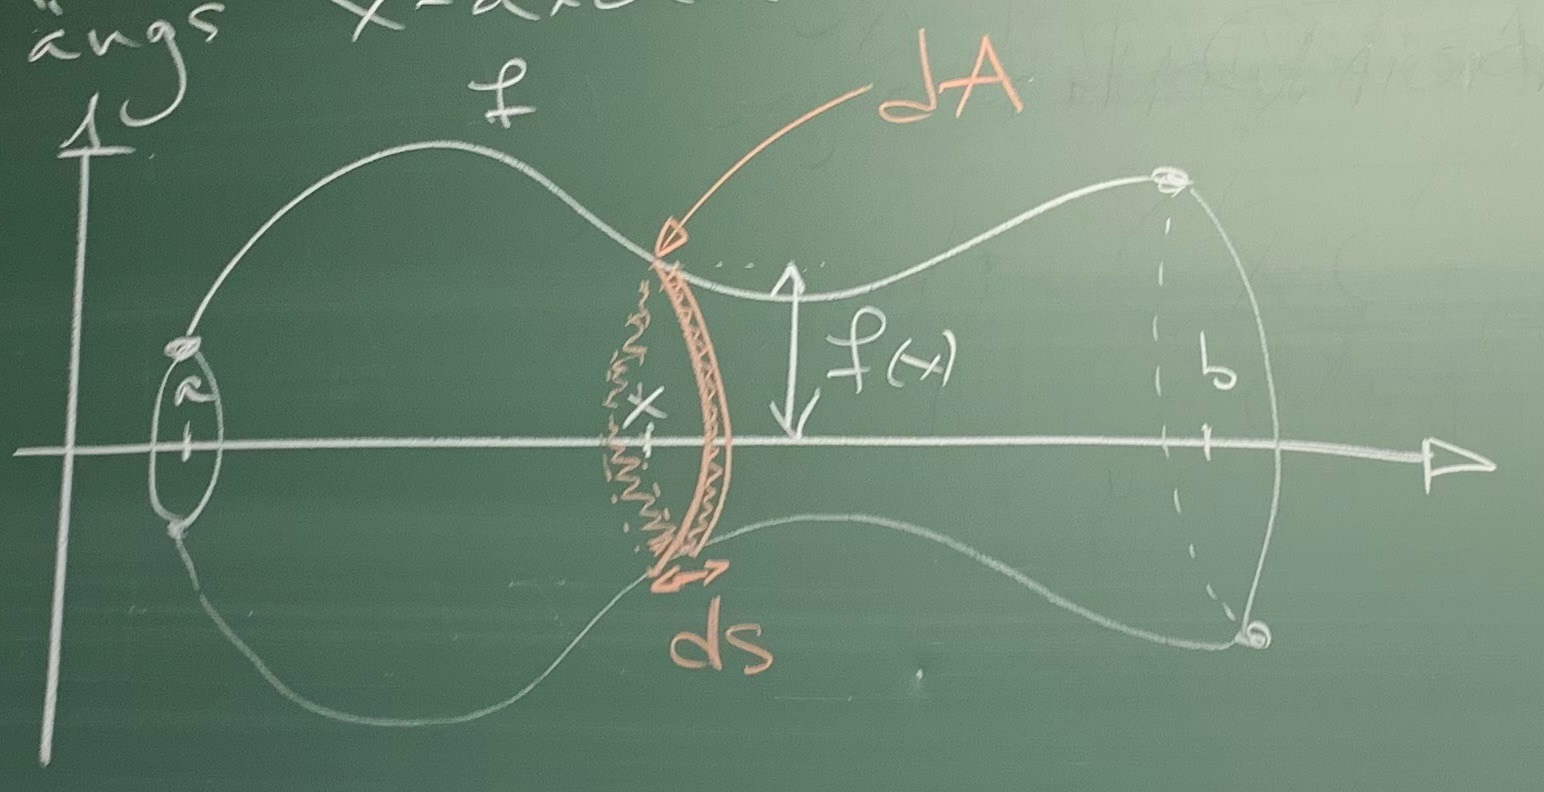
\includegraphics[scale=0.1]{lessons/lesson19/imgs/img12.jpg}\\
Måste hitta uttryck för area elementet $dA$ så att den totala mantelarean $A$ kan beräknas som $A=\int dA$.
Bandet med arean $dA$ kan "klippas upp" och tänkas som en rektangel med höjd $ds$ och längd $2\pi f(x)$, så:
\begin{equation*}
    dA=2\pi|f(x)|\, ds=
    2\pi|f(x)|\sqrt{1+(f^\prime(x))^2}\, dx
\end{equation*}
och allstå kan $A$ beräknas som
\begin{equation*}
    A=\int dA=2\pi\int_a^b|f(x)|\cdot\sqrt{1+(f^\prime(x))^2}\, dx
\end{equation*}